\section{System}
This section contains tests performed on the complete system after the code was deemed complete. To test the entire system, multiple nodes have to be setup and ready. The tests explained in this chapter were performed with a main node, and two sensor nodes.

The main node and sensor nodes have different tasks in the system, so the test parameters are different. Below is the tasks that were performed during the testing, for both node types.

\textbf{Sensor nodes} \\
\begin{itemize}
\item Send pair request if an ID is not found on the EEPROM.
\item Save node ID on EEPROM when an ID is received from main node.
\item When receiving a request, save the sender ID as parent, and send data back to this node. If a parent is already known, ignore this request.
\item When receiving acknowledgement of data from parent node, stop sending data and send requests.
\item When receiving data from a subnode, send acknowledgement to this subnode.
\item After sending acknowledgement, relay data to parent node until acknowledgement is received.
\item When a clear signal is received, clear parent and stop all actions. Relay clear to other nodes in the vicinity.
\end{itemize}


\subsubsection*{Main node}
\begin{itemize}
\item When receiving pair request, generate ID and send this to the node.
\item When user requests data in interface, send data requests.
\item When receiving data from subnode, save data and send acknowledgement to sender.
\item If all nodes have now sent data, save data in file and show user results of request. Send clear when file is saved to stop any action in the network.
\end{itemize}

The tests above covers the basic functionality of both main node and sensor nodes. In that order, they describe what the nodes should do from they start to a request is finished.
Testing these tasks can be done by observing a node that is part of the system, and test whether it does what it is supposed to. This requires multiple tests, as all nodes have to be observed at some point to determine wether the nodes do what they are supposed to do.

Due to the long range of the radio modules, relaying had to be tested using special code to ensure that a direct transmission between the main node and all sensor nodes. This meant that one of the sensor node were running code that ignored packets from the main node, to force that node into becoming a subnode of the other sensor node used in the test.

\subsubsection*{Results}
By monitoring sensor nodes while a request was underway, it was possible to see that the nodes reacted in the correct way to requests. First, by sending their own data to the parent node, whose ID was saved when the request arrived, and then stopping when an acknowledgement was received from the parent.

The sensor node then sent out requests, but with itself as the addresser. The other node received the request and then followed the same procedure as the first node. Upon receiving data, the first node relayed this data to the main node.

\begin{figure}[h!]
\centering
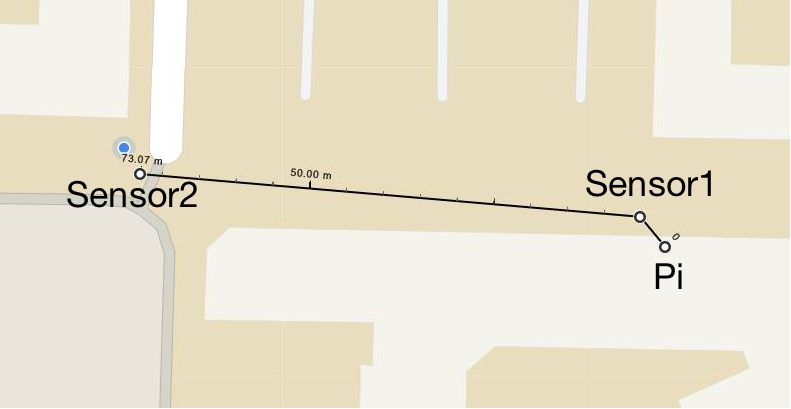
\includegraphics[width=1\textwidth]{chapters/test/figures/systest.png}
\caption{System test on map, showing nodes.}
\label{fig:systest}
\end{figure}

The main node now had data from all sensor nodes. This data was saved to a file, and clear requests were send out. The clear requests were then relayed from the first level sensor node to the second one and the request were complete.

This proved that the sensor nodes and main nodes completed their tasks. Testing showed an error in the implementation of exponential backoff, which made it possible for the delay to go out of bounds on the Arduino platforms. This was fixed after discovery.

Figure \ref{fig:systest} shows the setup of the test. The \texttt{Raspberry Pi} was inside the group room with both sensor nodes being outside. When started, \texttt{Sensor1} received the request from the Pi. This made  \texttt{Sensor1} send data back to the Pi and then send requests. \texttt{Sensor2} then send data to \texttt{Sensor1} which were then relayed to the Pi, which then cleared the system.
